\begin{center}
  \Large
  \textbf{BIOGRAFI PENULIS}
\end{center}

\addcontentsline{toc}{chapter}{BIOGRAFI PENULIS}

\vspace{2ex}

\begin{wrapfigure}{L}{0.3\textwidth}
  \centering
  \vspace{-3ex}
  % Ubah file gambar berikut dengan file foto dari mahasiswa
  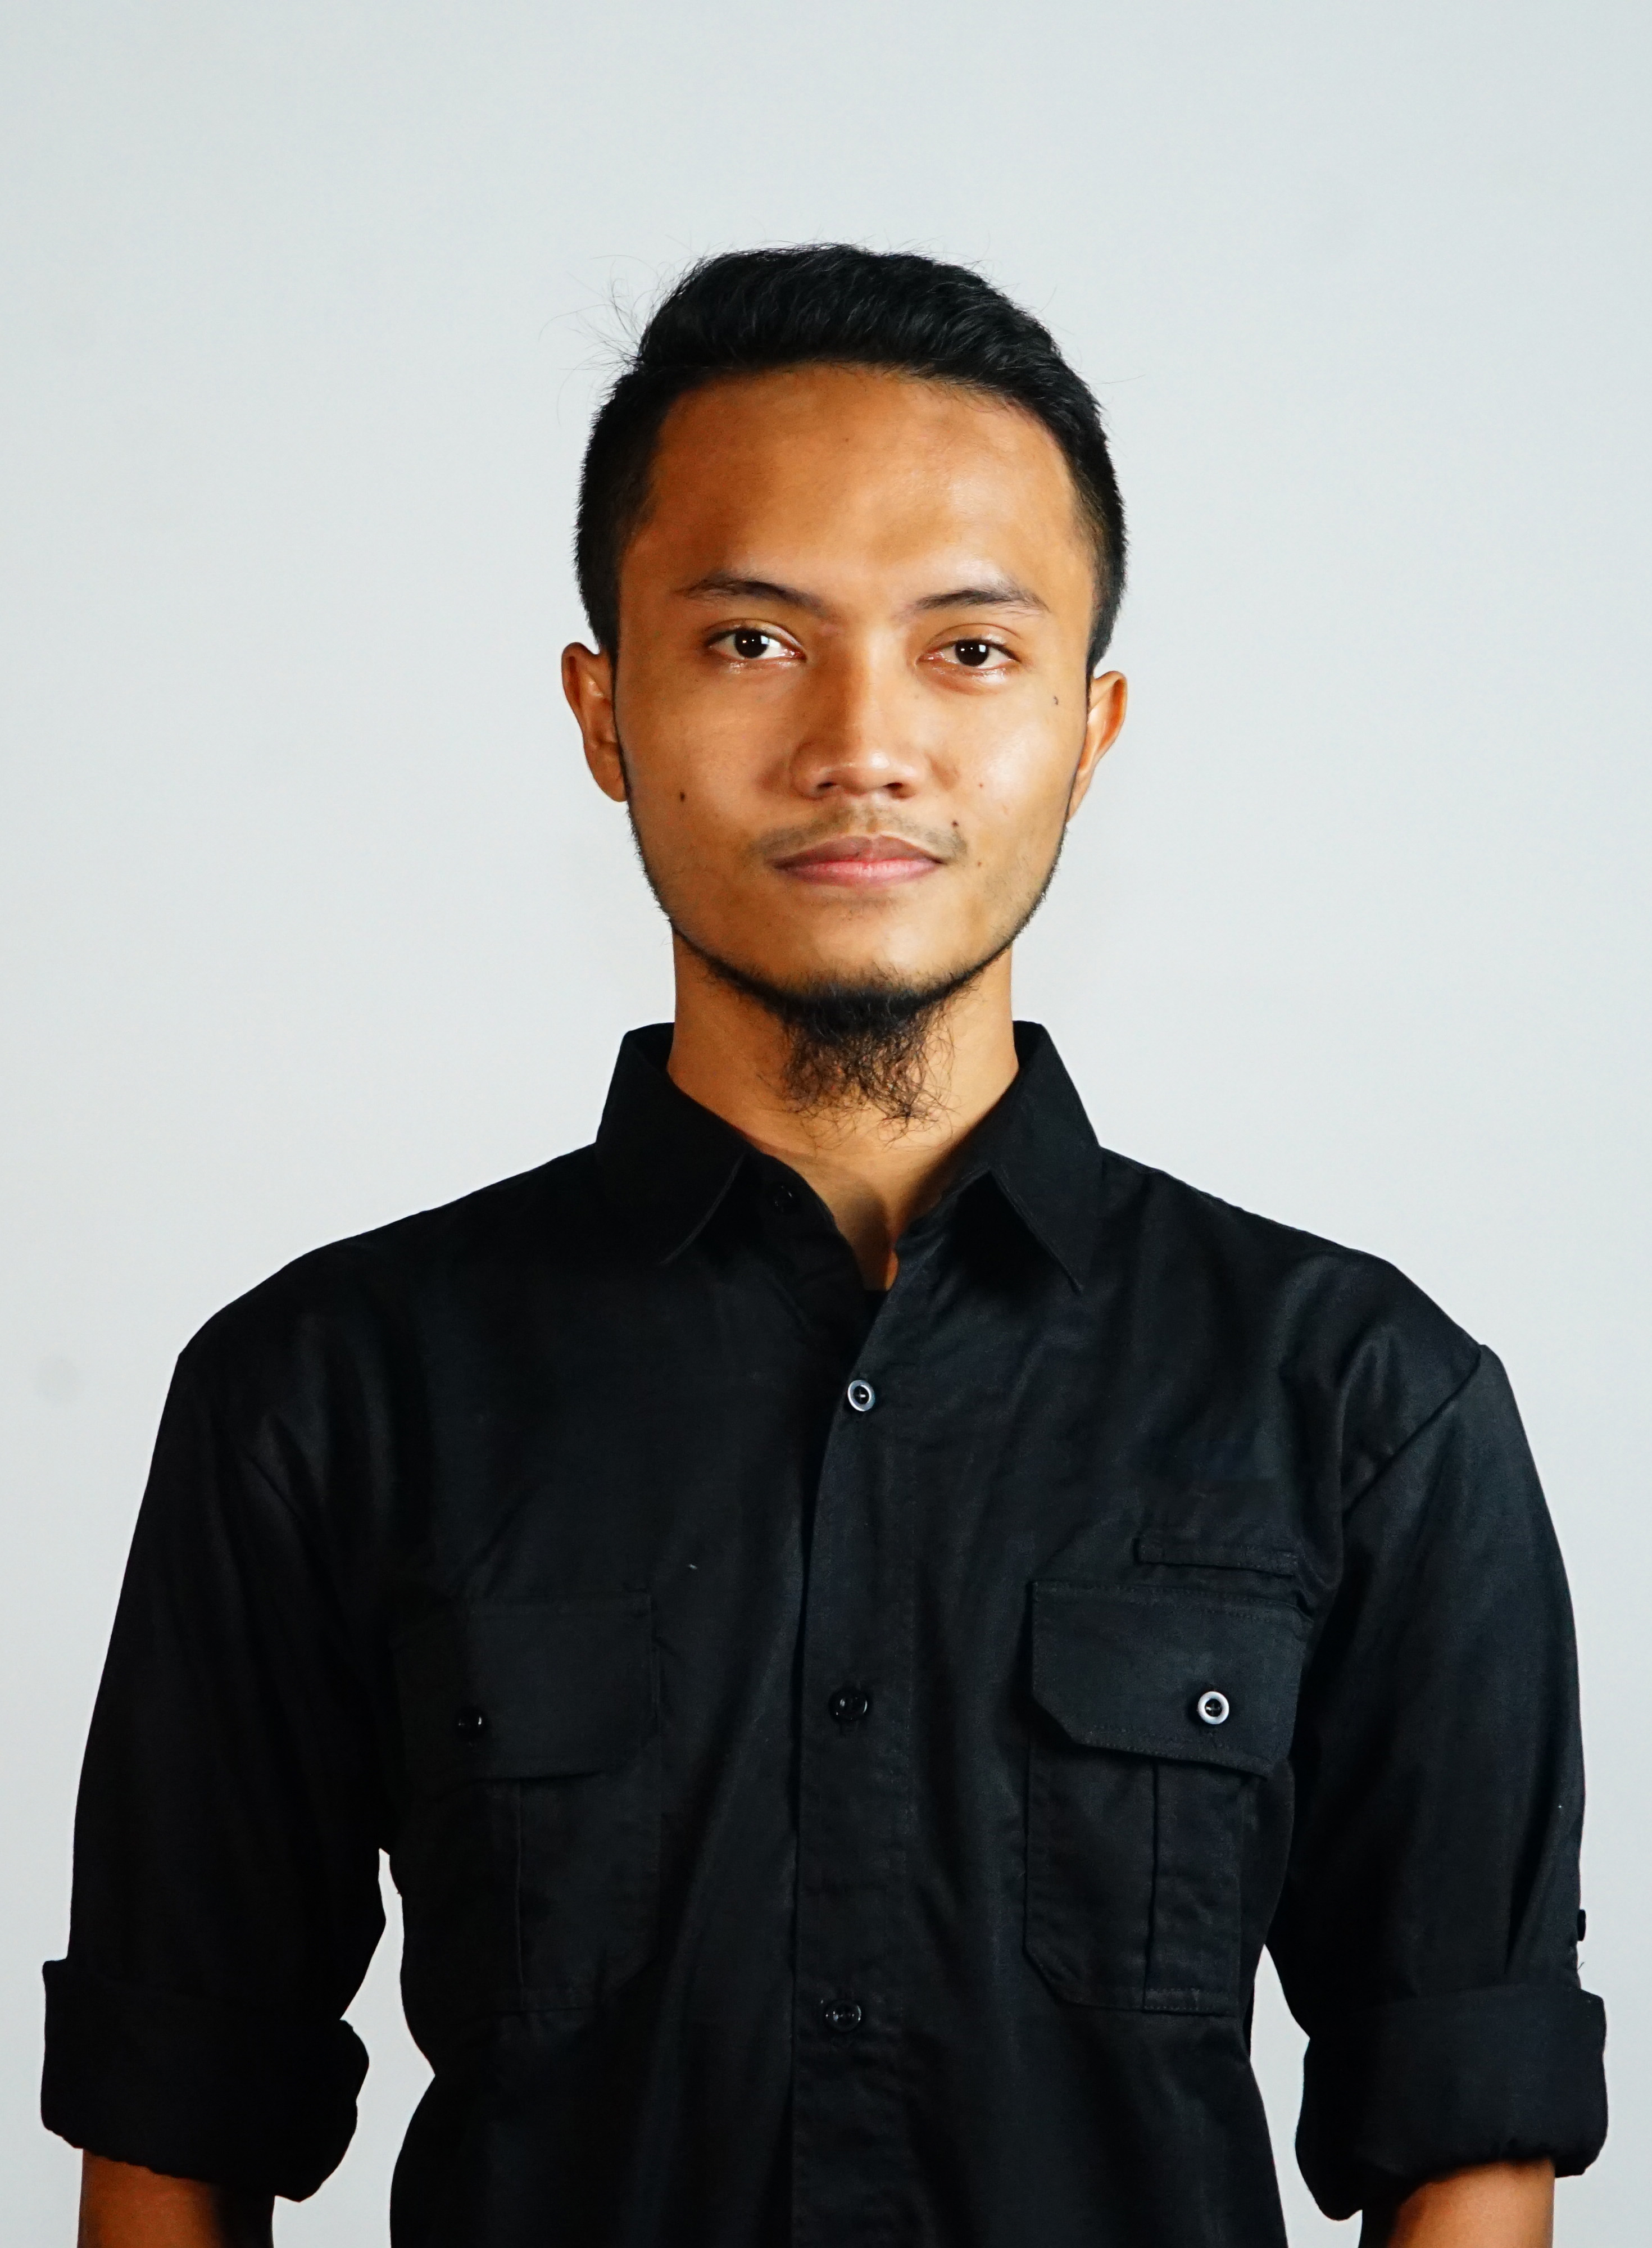
\includegraphics[width=0.3\textwidth]{gambar/biodimas.jpg}
  \vspace{-4ex}
\end{wrapfigure}

% Ubah kalimat berikut dengan biografi dari mahasiswa
\name{}, atau biasa dipanggil Dimas, lahir di Bondowoso, Jawa Timur pada 5 Desember 2000. Merupakan anak kedua dari dua saudara. Penulis lulus dari SMP Negeri 1 Bondowoso dan melanjutkan ke SMA Negeri 2 Bondowoso. Penulis melanjutkan ke jenjang strata satu di Departemen Teknik Komputer Fakultas Teknologi Elektro dan Informatika Cerdas Institut Teknologi Sepuluh Nopember (ITS). Dalam masa kuliah, penulis tertarik dengan jaringan komputer, pengembangan Robotika dan \emph{Internet of Things} (IoT), \emph{Web Design} dan UI/UX. Penulis pernah aktif menjadi salah satu anggota kru hingga menjadi \emph{quality control} dari ITS TV (2020-2023) dan aktif dalam organisasi mahasiswa yaitu anggota staf Departemen Komunikasi dan Informasi (Kominfo) dan Wakil Departemen \emph{Relation and Comunication} HIMATEKKOM ITS (2021-2023). Pada penelitian akhir ini, penulis memilih mengembangkan penelitian di bidang \emph{Machine Learning} yang berfokus pada Visi Komputer dalam lingkup olahraga pada treadmill. Bagi pembaca yang memiliki kritik, saran, atau pertanyaan mengenai tugas akhir ini dapat menghubungi penulis melalui surel dimas.adityamf@gmail.com.

